\begin{pa} \label{PA:10.5} Suppose you are driving around in the
  $xy$-plane so that our position is given by the vector-valued
  function 
  $$
  \vr(t) = \langle x(t), y(t) \rangle = \langle 2-t^2, t^3 + 1\rangle.
  $$
  The path we take is shown on the left of Figure
  \ref{F:10.5.preview}.  

  \begin{figure}
    \begin{center}
      \includegraphics{figures/fig_10_5_preview_r.eps}
      \hspace*{20pt}
      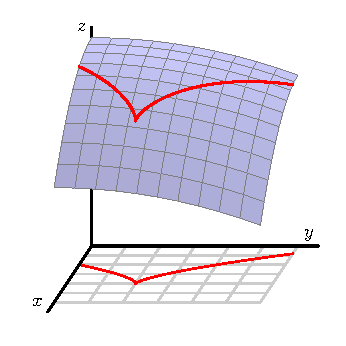
\includegraphics{figures/fig_10_5_preview_h.eps}
    \end{center}
    \caption{Our position in the plane and the corresponding temperature.}
    \label{F:10.5.preview}
  \end{figure}
  Suppose, furthermore, that
  the temperature at a point in the plane is given by
  the function
  $$
  T(x,y) = 10 - \frac12x^2 -\frac15y^2,
  $$
  as shown on the right of Figure \ref{F:10.5.preview}.  Therefore, as
  time passes, your position $(x(t), y(t))$ changes, and, as your position
  changes, the temperature $T(x,y)$ changes.
  
  \ba
\item What is your position at time $t=1$;  that is, what are the $x$-
  and $y$-coordinates of your location?
\item What is the temperature at this point?
\item Write the differential $dT$ in terms of $dx$ and $dy$ at this
  point. 
\item With what velocity are you traveling at $t=1$?
\item Suppose time increases a little bit to $t=1.1$.  This
  represents a change in time of $dt=0.1$.  Use the velocity you
  determined in the last part of this activity to estimate the change
  $dx$ in your $x$-coordinate and the change $dy$ in your
  $y$-coordinate.
\item Use differentials to estimate the corresponding change in
  temperature $dT$.

  \ea

\end{pa} 
\afterpa 